\chapter{Enfoques computacionales a la calidad de informaci\'on en Wikipedia}

En el cap\'itulo anterior, se explicaron distintos aspectos relacionados a la calidad de la informaci\'on en Wikipedia. En este cap\'itulo abordaremos diferentes enfoques computacionales que capturan estos aspectos de calidad, los cuales podemos dividir en \emph{m\'etricas de calidad}, \emph{identificaci\'on de art\'iculos destacados}, \emph{detecci\'on de fallas en Wikipedia} y \emph{visualizaci\'on}. Cada uno de estos permite obtener, a trav\'es de diferentes formas y m\'etodos, indicadores que marcan si un art\'iculo de la Wikipedia en Ingl\'es contiene caracter\'isticas relacionadas a la calidad.

Como principal prop\'osito, en este cap\'itulo se mostrar\'an definiciones y ejemplos de cada uno de los enfoques, adem\'as, tambi\'en se presentar\'an caracter\'isticas y tareas puntuales para determinar aspectos de calidad en los art\'iculos de Wikipedia.

\emph{Organizaci\'on del cap\'itulo.} La subsecci\'on 3.1 presenta una definici\'on formal de \emph{m\'etricas de calidad} y se diferencia del concepto de \emph{medida}. Adem\'as se presentan diversas m\'etricas utilizadas en trabajos previos. La subsecci\'on 3.2, se enfoca en la tarea de identificar art\'iculos destacados y las caracter\'isticas que poseen para diferenciarlos del resto de los art\'iculos. La subsecci\'on 3.3 describe algunas fallas de calidad detectadas en los art\'iculos de Wikipedia y c\'omo los usuarios interact\'uan con las etiquetas de limpieza. La subsecci\'on 3.4 (falta definir).

\section{M\'etricas de calidad}

Actualmente, se ha puesto especial inter\'es en la definici\'on de m\'etricas de calidad sobre los art\'iculos de Wikipedia a trav\'es de diferentes criterios, marc\'andolo como un aspecto ampliamente importante dentro del \'area inform\'atica.

Hoy en día, se carece de una definici\'on formal de lo que una m\'etrica es, sin embargo, formularemos una definici\'on formal que se ajuste a lo que una m\'etrica es realmente.

En una primera instancia, definiremos y diferenciaremos los conceptos de \emph{medida} y \emph{m\'etrica}, los cuales podr\'ian parecer similares.

La estimaci\'on de la calidad de un art\'iculo de Wikipedia, se vincula directamente con la identificaci\'on y valoraci\'on de distintas \emph{propiedades} que este art\'iculo puede tener. En este contexto, en este trabajo diferenciaremos aquellas propiedades que son directamente \emph{medibles} de un art\'iculo de Wikipedia particular, que referenciaremos como \emph{medidas de calidad}, de aquellas que se definen en forma abstracta, como la \emph{combinaci\'on} de una o m\'as propiedades del art\'iculo y que llamaremos \emph{m\'etricas de calidad}. Por ejemplo, Stvilia ~\cite{StvTwSmGa:05} en su trabajo, define la \emph{completitud} como una m\'etrica de calidad que se calcula de la siguiente manera:


\begin{equation}
 \label{eq:ec1}
\begin{split}
& 0.4 \ \times \ Cantidad \ de \ v\acute{\imath}nculos \ internos \ rotos \ + \ 0.4 \ \times \ Cantidad \ interna \ de \\
& v\acute{\imath}nculos + \ 0.2 \ \times Longitud \ del \ art\acute{\imath}culo
\end{split}
\end{equation}

En este caso, la m\'etrica \emph{completitud} est\'a compuesta por las medidas: \emph{cantidad de v\'inculos internos rotos}, \emph{cantidad interna de v\'inculos} y \emph{longitud del art\'iculo}.

Las propiedades de un art\'iculo, tendr\'an asociadas un \emph{sistema de valoraci\'on} el cual, dado un documento, le hace corresponder el \emph{valor} (num\'erico) que dicho documento tiene para esta propiedad. M\'as formalmente, si $p$ es una propiedad cualquiera, su sistema de valoraci\'on $p^\sigma$ es una regla (o funci\'on) que asocia a cada art\'iculo de Wikipedia un valor num\'erico correspondiente con dicha propiedad $p$. Estas ideas son expresadas en notaci\'on matem\'atica en la siguiente definici\'on.
\\

\textbf{Definici\'on 1: Sistema de Valoraci\'on.} Sea $p$ una propiedad, $D$ el conjunto de art\'iculos de Wikipedia, y $N$ un valor de tipo num\'erico (por ejemplo el conjunto de los enteros ($\mathbb{Z}$) o el conjunto de los reales ($\realset$)). El \emph{sistema de valoraci\'on} $p^\sigma$ de la propiedad $p$, es una funci\'on: $$p^\sigma: D \rightarrow N$$

tal que para todo art\'iculo de Wikipedia $d \in D$, si $p^\sigma(d)=v$, $v$ representa el valor correspondiente a la propiedad $p$ en el art\'iculo $d$. Luego, diremos que ``$v$ es la \emph{valoraci\'on} de $d$ en la propiedad $p$'' o directamente que ``la propiedad $p$ de $d$ es $v$''. \label{def1}

Las propiedades m\'as sencillas de analizar son aquellas cuyos sistemas de valoraci\'on consisten en un \emph{instrumento} o \emph{m\'etodo} que obtienen el valor asociado con un documento directamente de una \emph{medici\'on} (\emph{aplicaci\'on}) directa del instrumento sobre el documento. En estos casos, los sistemas de valoraci\'on son en realidad \emph{sistemas de medici\'on} y a estas propiedades b\'asicas las denominaremos \emph{medidas de calidad}.

As\'i, por ejemplo, la \emph{longitud} de un art\'iculo, su \emph{riqueza de vocabulario}, el \emph{n\'umero de revisiones} que un art\'iculo ha tenido desde su revisi\'on, o la \emph{edad} del art\'iculo, son propiedades a las que se le puede asociar el valor correspondiente mediante la simple \emph{medici\'on directa} sobre el art\'iculo utilizando el instrumento (programa) adecuado que realiza el c\'alculo correspondiente. A modo de ejemplo, la biblioteca
NLTK\footnote{Biblioteca NLTK. www.nltk.org} (por Natural Language Toolkit) provee una colecci\'on interesante de programas en Python que implementan ese
tipo de instrumentos o medidas.

As\'i, por ejemplo, si $d$ es un art\'iculo arbitrario de Wikipedia, y $long$ representa la medida de calidad \emph{longitud} del
art\'iculo, $long^\sigma(d)$ representar\'a la longitud efectiva del art\'iculo $d$ (medido en bytes o palabras).

Adem\'as de estas propiedades b\'asicas, un art\'iculo puede tener otras propiedades m\'as abstractas, cuya definici\'on y valoraci\'on no
 son tan directas como en las medidas de calidad, y que en el contexto  de este trabajo llamaremos \emph{m\'etricas de calidad}.

Una m\'etrica de calidad, al igual que una medida de calidad, tambi\'en es una propiedad que permite asociar un valor num\'erico a un art\'iculo
de Wikipedia. Sin embargo, en este caso, la propiedad a ser cuantificada se define en base a otras propiedades del art\'iculo que
pueden estar dadas como medidas de calidad o m\'etricas de calidad. Es importante observar que mientras el valor de una propiedad
especificado por una medida es ``objetivo'', en el sentido que s\'olo depende de un instrumento de medici\'on apropiado de la caracter\'istica
a medir, las m\'etricas son ``estimaciones subjetivas'' ya que dependen de las propiedades particulares utilizadas en su definici\'on
y de la forma elegida para combinarlas.

Para ver m\'as claramente estas ideas, consideremos el caso de la m\'etrica  de calidad \emph{grado de informaci\'on}, que busca
capturar el grado de informaci\'on contenido en un art\'iculo. Esta caracter\'istica/m\'etrica es referenciada en Ingl\'es como la propiedad (abstracta) ``\emph{informativeness}''. Una primera aproximaci\'on para estimar la m\'etrica \emph{grado de informaci\'on}, podr\'ia consistir en basarla en la medida  \emph{longitud}, con el argumento de que a mayor longitud del art\'iculo, se supone que \'este contiene m\'as cantidad de informaci\'on. Un enfoque m\'as elaborado por otra parte, podr\'ia considerar que no s\'olo la informaci\'on textual es importante, sino que tambi\'en es muy \'util
considerar la medida de la \emph{cantidad de im\'agenes} que se muestran en el art\'iculo, tomando como lema la frase ``una imagen
vale m\'as que mil palabras''. En este ejemplo sencillo, es f\'acil observar que la decisi\'on de cu\'ales ser\'an las propiedades (medidas en
este caso) a utilizar y de la forma de ponderarlas y combinarlas, constituyen un aspecto \emph{subjetivo} y dependiente de la persona
encargada de definir la m\'etrica.

Una vez introducidas informalmente las similitudes y diferencias entre medidas y m\'etricas de calidad podemos decir, m\'as formalmente,
que una m\'etrica de calidad es una propiedad de un art\'iculo cuyo sistema de valoraci\'on se basa en otras propiedades de dicho
art\'iculo, las cuales a su vez pueden ser medidas o m\'etricas de calidad. Estas ideas son expresadas en notaci\'on matem\'atica en la
siguiente definici\'on.
\\

\textbf{Definici\'on 2: M\'etrica de calidad.} Sea $\mathcal{P}= \{p_1,p_2,\ldots,pn\}$ un conjunto de propiedades (medidas o m\'etricas de calidad) de un art\'iculo de Wikipedia y sean $D$ y $N$ los conjuntos introducidos en la Definici\'on 1.
Una \emph{m\'etrica de calidad} $\mu_\mathcal{P}$, definida en base a las propiedades en
 $\mathcal{P}$, es una propiedad cuyo sistema de valoraci\'on es una funci\'on: $$ \mu_\mathcal{P}^\sigma: D \rightarrow N$$ tal que para todo art\'iculo de
Wikipedia $d \in D$, si $\mu_\mathcal{P}^\sigma(d)= v$, $v$ representa el valor de la propiedad $\mu$ en el art\'iculo $d$, el
cual es computado en base a los valores $p_1^\sigma(d),p_2^\sigma(d),\ldots, p_n^\sigma(d)$, para todo $p_i \in \mathcal{P}$.

De la definici\'on anterior, es directo observar que la definici\'on de una m\'etrica de calidad, admite el uso de otras m\'etricas de calidad.
Por lo tanto, en estos casos, su valoraci\'on se resolver\'a en forma recursiva, hasta que la propiedad a valorar sea una medida de
calidad, cuyo valor se determina directamente por un sistema de medici\'on. En este sentido, es importante notar que la diferencia
antes mencionada entre \emph{medici\'on} (representada por una \emph{medida de calidad}) y \emph{evaluaci\'on estimativa}
(representada por una \emph{m\'etrica de calidad}) es similar a la que en Ingl\'es se realiza entre los t\'erminos \emph{measurement} y
\emph{assessment}.

Para clarificar los conceptos antes introducidos, continuemos con el ejemplo de la m\'etrica de calidad \emph{grado de informaci\'on} que representa el grado de informaci\'on (\emph{informativeness}) contenida en un art\'iculo de Wikipedia.

Si la m\'etrica \emph{grado de informaci\'on} (que abreviaremos $info$), es estimada como la suma de la \emph{longitud} del
art\'iculo (abreviada $long$) y el doble de la \emph{cantidad de im\'agenes} del art\'iculo (abreviada $cim$), es decir,

\begin{center}
\emph{grado de informaci\'on} $=$ \emph{longitud} $+$ $2$ $\times$
\emph{cantidad de im\'agenes}
\end{center}

la valoraci\'on del \emph{grado de informaci\'on} de un art\'iculo $d$ ($info^\sigma(d)$), se obtiene de la siguiente manera:

$$info^\sigma(d) = long^\sigma(d) + 2 \times cim^\sigma(d)$$

A modo de ejemplo, un art\'iculo de Wikipedia $d$ cuya longitud es de 126 palabras ($long^\sigma(d) = 126$), y que contiene 15 im\'agenes
($cim^\sigma(d) = 15$) tendr\'a un grado de informaci\'on estimado de 156 ($info^\sigma(d) = 156$)

Un ejemplo destacado, que plantea una mirada diferente, es el que podemos apreciar en las 7 m\'etricas de calidad aplicadas a art\'iculos de Wikipedia creadas por Stvilia ~\cite{StvTwSmGa:05}. Podemos ver como cada una de estas m\'etricas est\'a definida en base a una o varias medidas como se explic\'o anteriormente.
\begin{enumerate}
	\item \emph{Autoridad / Reputaci\'on} = 0.2 $\times$ Cantidad editores \'unicos + 0.2 $\times$ Cantidad Total de ediciones + 0.1 $\times$
Conectividad\footnote{Cantidad de art\'iculos conectados a un art\'iculo particular a trav\'es de editores frecuentes} + 0.3 $\times$ Cantidad de veces que se revirti\'o + 0.2 $\times$ Cantidad v\'inculos externos + 0.1 $\times$ Cantidad de ediciones de usuarios registrados + 0.2 $\times$ Cantidad de ediciones de usuarios an\'onimos.
	\item \emph{Completitud} = 0.4 $\times$ Cantidad de v\'inculos internos rotos + 0.4 $\times$ Cantidad interna de v\'inculos + 0.2 $\times$ Longitud del art\'iculo
	\item \emph{Complejidad} = Puntuaci\'on de legibilidad de Flesch\footnote{Prueba de legibilidad de Flesch. \\ https://es.wikipedia.org/wiki/Prueba\_de\_legibilidad\_de\_Flesch-Kincaid}
	\item \emph{Informatividad} = 0.6 $\times$ Informaci\'on de Ruido\footnote{1- (La cuantificaci\'on del t\'ermino / vector de token antes de stemizar y aplicar palabra de paro) / (longitud del documento antes de ser procesado)} - 0.6 $\times$ Diversidad\footnote{(Cantidad de editores \'unicos / Cantidad total de ediciones} + 0.3 $\times$ Cantidad de Im\'agenes
	\item \emph{Consistencia} = 0.6 $\times$ Ediciones compartidas por el administrador\footnote{Cantidad de ediciones del administrador /
Cantidad total de ediciones} + 0.5 $\times$ Edad
	\item \emph{Actualidad} = Actualidad\footnote{El tiempo entre la fecha de volcado y la fecha de la \'ultima actualizaci\'on del art\'iculo medido en d\'ias)}
	\item \emph{Volatilidad} = Tiempo medio de reversiones
\end{enumerate}

Las nombradas m\'etricas fueron calculadas en cada art\'iculo de Wikipedia sobre un total de 236 art\'iculos destacados y 834 art\'iculos aleatorios y luego agrupados y clasificados de acuerdo a las medidas previamente mencionadas.

Los resultados mostrados luego de la aplicaci\'on de las mismas, mostraron exitosamente que pueden distinguir art\'iculos destacados del resto de los art\'iculos.

Otro enfoque relacionado con las m\'etricas que presenta un planteamiento distinto, podemos verlo en el trabajo de ~\cite{InDuRoSe:12}, en el cual se construyen grafos capturando diferentes aspectos. En dicha investigación se plantean las siguientes m\'etricas:

\begin{enumerate}
	\item \emph{Coeficiente de agrupamiento}: representa el promedio de los coeficientes de agrupamientos de los nodos. Para un nodo particular \emph{i} se define de la siguiente manera:


\begin{equation}
\label{eq:ecej2}
	C{_i} = \frac {e{_i}} {[\frac {k{_i}(k{_i}-1)} {2}]}
\end{equation}

Donde e$_{i}$ es el n\'umero de v\'inculos entre vecinos de \emph{i}. \\
k$_{i}$ es el n\'umero de vecinos del nodo \emph{i}.\\
{k$_{i}$(k$_{i}$-1)} / {2} es el n\'umero de v\'inculos cuando los vecinos est\'an completamente conectados.

	\item \emph{Longitud de trayectoria media}: representa la media del n\'umero m\'inimo de aristas que tiene que ser atravesado para llegar a un nodo desde todos los nodos de la red. La longitud de trayectoria media para un nodo \emph{i} se define de la siguiente manera.

\begin{equation}
\label{eq:ecej2.1}
Pi = \sum_{k=1}^{n} \frac {m_{k}} {n}
\end{equation}

Donde m$_{k}$ representa el n\'umero m\'inimo de nodos que deben ser atravesados para alcanzar el nodo \emph{i} desde el nodo \emph{k} y \emph{n} es el n\'umero total de nodos en la red.

Esta m\'etrica mide el n\'umero promedio de intermediarios entre dos nodos cualquiera en la red buscando el camino m\'as corto. Cuanto menor sea el valor de esta m\'etrica de una red, m\'as cerca se encuentran los nodos, representando una red con pocos agujeros estructurales.
\end{enumerate}

Como resultado de la aplicaci\'on de estas m\'etricas, se confirma que los agujeros estructurales en los grafos generados est\'an directamente asociados con la calidad.

Otro trabajo de investigaci\'on, realizado por  ~\cite{AnLih:04}, muestra una manera diferente de plantear las m\'etricas. En su lugar, mide la calidad de los art\'iculos a trav\'es del concepto \emph{``reputaci\'on'}' definido por dos m\'etricas que mostraremos a continuaci\'on. En particular, estas s\'olo se calculan sobre metadatos y no sobre el contenido de los art\'iculos.

\begin{enumerate}
\item \emph{Rigor}:  este aspecto est\'a marcado por el n\'umero total de ediciones de un art\'iculo. Como premisa, se supone que un art\'iculo que tiene muchas ediciones posee un tratamiento mucho mayor y m\'as profundo.

\item \emph{Diversidad}: esta caracter\'istica est\'a determinada por n\'umero total de usuarios \'unicos que editaron un art\'iculo particular. En otras palabras, se intenta ver la cantidad de diferentes usuarios (an\'onimos o registrados) que se expresaron en el mismo art\'iculo.
\end{enumerate}

Otros trabajos han planteado diferentes enfoques a la hora de abordar el tema m\'etricas. Veamos a continuaci\'on como se trataron y estudiaron.

Un enfoque destacado es planteado por Stvilia ~\cite{StvTwSmGa:05} en el que define 7 m\'etricas: autoridad, completitud, complejidad, informatividad, consistencia, precisi\'on y volatilidad. Ellas pueden ser evaluadas autom\'aticamente y probadas sobre una muestra representativa de la Wikipedia en Ingl\'es.

A trav\'es del an\'alisis estad\'istico de caracter\'isticas de art\'iculos aleatorios y sus metadatos de los historiales de edici\'on, se crearon perfiles de 19 medidas de calidad. Dichos perfiles fueron evaluados por redundancia usando la t\'ecnica de an\'alisis de factor exploratorio ~\cite{JoWi:98}, luego se construyeron las 7 m\'etricas de calidad. Por \'ultimo, se evaluaron las mismas midiendo la habilidad de capturar la varianza  de la calidad de la informaci\'on de la colecci\'on de datos, a trav\'es de agrupamientos y clasificaci\'on de perfiles etiquetados de las m\'etricas de calidad de las caracter\'isticas y art\'iculos aleatorios.

Estas m\'etricas de la calidad de la informaci\'on deb\'ian, como objetivo principal, generar estimaciones que capturen una porci\'on importante de la varianza de un art\'iculo y al mismo tiempo evitar sesgos y redundancias.

Otro enfoque, considerado como el conjunto m\'as relevante de \emph{m\'etricas de calidad} para el contexto de Wikipedia, fue propuesto por ~\cite{ZhuGau:00}, en el cual, para medir la calidad de las p\'aginas Web definieron las siguientes m\'etricas.
\begin{itemize}
\item \emph{Actualidad:} medido como el tiempo de actualizaci\'on de una p\'agina (respecto a la fecha actual).
\item \emph{Radio de informaci\'on a ruido:} computado como la relaci\'on entre la longitud total de los items del \'indice por sobre el tama�\~no de la p\'agina.
\item \emph{Disponibilidad:} computada como la relaci\'on entre el n\'umero de v\'inculos rotos y la cantidad de v\'inculos en toda la p\'agina.
\item \emph{Cohesi\'on:} el grado en el cual el contenido de una p\'agina se centra en un tema. Esto fue alcanzado gracias al directorio ontol\'ogico Magellan.
\item \emph{Autoridad:} m\'etrica basada en la revisi\'on de la vida de Internet de Yahoo, asignando valores entre 2 y 4 y el valor 0 en el caso que no haya sido revisada.
\item \emph{Popularidad:} estimada por el n\'umero de p\'aginas Web que citan a una p\'agina Web particular. Las puntuaciones fueron obtenidas de el buscador Altavista.
\end{itemize}

En el enfoque presentado por ~\cite{InDuRoSe:12}, se utiliza el m\'etodo de an\'alisis de redes sociales  ~\cite{WaFa:94}, en el cual plantearon a Wikipedia como una red de conocimiento que surge del conjunto de relaciones e interacciones entre los art\'iculos y los usuarios ~\cite{StaRD:00, KakSor:02}. En primer lugar, definieron una red de usuarios, donde cada nodo denota un usuario y cada relaci\'on entre ellos representa un art\'iculo com\'un al que han contribuido. Tambi\'en, existe otro grafo que se llama ``red de art\'iculos'' donde cada nodo representa un art\'iculo y cada enlace entre ellos representa un contribuidor com\'un. Ambas redes, con estructuras totalmente diferentes, capturan diferentes aspectos de interacci\'on, colaboraci\'on de la informaci\'on en la primera nombrada e informaci\'on tem\'atica en la segunda.
Como resultado del an\'alisis, se revela que clusters de art\'iculos de alta calidad se encuentran agrupados en lugares con agujeros estructurales.

Otro enfoque, explicado también en párrafos anteriores, se muestra en ~\cite{DavGf:03, UzSp:05}, donde se utilizaron dos m\'etricas: \emph{coeficiente de agrupamiento} y \emph{longitud de trayectoria media} para identificar la estructura de la red y, m\'as espec\'ificamente, la presencia o ausencia de un agujero estructural. La primera nombrada es  el promedio de los coeficientes de clustering de los nodos (grado de agrupamiento en que los nodos tienden a agruparse), mientras que la segunda es la media del n\'umero m\'inimo de aristas que tiene que ser atravesado para llegar a \'el desde todos los nodos de la red.

En el trabajo presentado por ~\cite{AnLih:04}, e introducido como ejemplo anteriormente, se mide la ``reputaci\'on'' de los art\'iculos a trav\'es de dos m\'etricas bien definidas, \emph{rigor} y \emph{diversidad}. La primera representa el n\'umero total de ediciones de un art\'iculo, que supone que a mayor cantidad de ediciones se provee un tratamiento m\'as profundo del objeto de estudio, mientras que el segundo, el n\'umero total de usuarios \'unicos, marca la cantidad de ``voces'' diferentes en el tema. Estos valores s\'olo fueron obtenidos considerando metadatos de los art\'iculos en cuesti\'on, sin considerar el contenido de los mismos. Para calcularlos se defini\'o un conjunto de temas de enciclopedia, los cuales son considerados ejemplares exactos y completos, contra los cuales se compararon los resultados obtenidos. Dichos resultados indican que hay una relaci\'on entre la historia del ``borrador del art\'iculo'' y las noticias de la actualidad.

Por otra parte, con el fin de medir la calidad de la informaci\'on basado en informaci\'on factual, en ~\cite{LeVoErFeCaHoGrr:12}, un enfoque diferente, se proponen tres enfoques: (i) el uso de simples estad\'isticas acerca de los hechos obtenidos de un texto, (ii) explotaci\'on de la informaci\'on relacional contenida en los hechos, y (iii) explotaci\'on de las relaciones sem\'anticas como meronimia y hiperonimia. Posteriormente, se propusieron para el primer enfoque caracter\'isticas estad\'isticas muy sencillas sobre hechos con el fin de determinar la capacidad informativa de un documento. Estas caracter\'isticas, que en ~\cite{LeVoErFeCaHoGrr:12} son nombradas como caracter\'isticas basadas en la frecuencia de hechos, son el antecedente m\'as cercano y la base para la mayor\'ia de las propuestas presentadas en \'este trabajo. Dichas caracter\'isticas ser\'an descritas en las pr\'oximas secciones con el fin de hacer m\'as f\'acil la comprensi\'on del concepto  ``soporte factual externo''.

Las caracter\'isticas basadas en la frecuencia de hechos s\'olo requieren informaci\'on sobre el n\'umero de hechos obtenidos por un proceso de extracci\'on de informaci\'on a partir de un recurso textual. Por ejemplo, si \emph{t} es un recurso textual arbitrario (un p\'arrafo, un documento, un corpus), y $F_{t}$ es la colecci\'on de hechos extra\'idos de \emph{t} por un m\'etodo extractor de informaci\'on arbitrario IE, se calcula directamente la cantidad de hechos de \emph{t}, denotado $F_{c}$(\emph{t}). Este es simplemente definido como el n\'umero total de hechos obtenidos de \emph{t} por IE, $f_{c}$ (t) = |$F_{\emph{t}}$|. Obviamente, la cantidad de hechos depende directamente del tama\~no del recurso textual \emph{t}, por lo que generalmente se normaliza de acuerdo al tama\~no de \emph{t}. Esta cantidad es referenciada en ~\cite{LeVoErFeCaHoGrr:12}, como la densidad factual de \emph{t}, y denota $f_{d}$ (\emph{t}). En ese caso, si \emph{size(t)} es una medida destinada a cuantificar el tama\~no de \emph{t}\footnote{Por ejemplo, podr\'ia ser el n\'umero de palabras o frases en \emph{T} o la longitud en n\'umero de caracteres de \emph{t}.}, la densidad factual de \emph{t}, se define como $f_{d}$ (\emph{t}) = $f_{c}$ (\emph{t}) / \emph{size(t)}.

Como se detallar\'a mas adelante, los hechos de la colecci\'on $F_{\emph{t}}$  se pueden utilizar para calcular el soporte factual externo de \emph{t}, donde t corresponde a un art\'iculo de Wikipedia.

En relaci\'on al uso de la informaci\'on ``externa'' para evaluar la calidad de la informaci\'on de un documento, vale la pena mencionar el trabajo de ~\cite{JuGrLe:09} en el contexto de una tarea de ranking de credibilidad de un blog. All\'i, los enfoques para evaluar la credibilidad de los blogs se basan en una comparaci\'on directa contra un corpus validado de noticias referenciadas. No utilizan informaci\'on factual y el dominio es diferente al que dirigi\'o en el presente art\'iculo, pero pudimos ver algunas similitudes en la idea de utilizar recursos externos como ``soporte'' del contenido interno de los documentos.

Probablemente, uno de los enfoques m\'as relacionados con nuestra propuesta se present\'o en ~\cite{MaWa:10}. Su enfoque para medir soporte de documentos de texto se basa en el uso de hechos muy b\'asicos derivados de frases sustantivo-a-sustantivo de un documento. Estos hechos se comparan con los obtenidos a partir de la informaci\'on recuperada por un motor de b\'usqueda conocido (Bing).

\section{Identificaci\'on de art\'iculos destacados}

En Wikipedia existen distintas calificaciones para los art\'iculos de acuerdo a su calidad como art\'iculo enciclop\'edico. El concepto formalizado a trav\'es del nombre \emph{Art\'iculo Destacado} (Featured Article), desde ahora llamado FA, corresponde a los mejores art\'iculos que Wikipedia puede ofrecer, seg\'un lo determinado por los ``Wikipedians'', editores de Wikipedia.

El art\'iculo destacado es identificado en el sitio Web de Wikipedia a trav\'es del icono de una estrella de bronce en la esquina superior derecha como se mostr\'o en secciones anteriores. Adem\'as, si el art\'iculo, tambi\'en es destacado en otros idiomas, una estrella aparecer\'a seguido al v\'inculo del lenguaje en la lista \emph{''En otros idiomas''}, posicionada del lado izquierdo de la p\'agina Web.

A modo de ejemplo, el art\'iculo \emph{''United States Bicentennial coinage''} (Monedas del Bicentenario de Estados Unidos), plasmado en la figura ~\ref{fig:usbicoinage}, corresponde a un art\'iculo destacado. El mismo trata acerca de monedas emitidas entre los a\~nos 1975 y 1976 en conmemoraci\'on a la independencia estadounidense. En el extremo superior derecho se remarca en rojo la estrella de bronce que indica la m\'axima calidad del art\'iculo en Wikipedia.

\begin{figure}[here]
	\begin{center}
		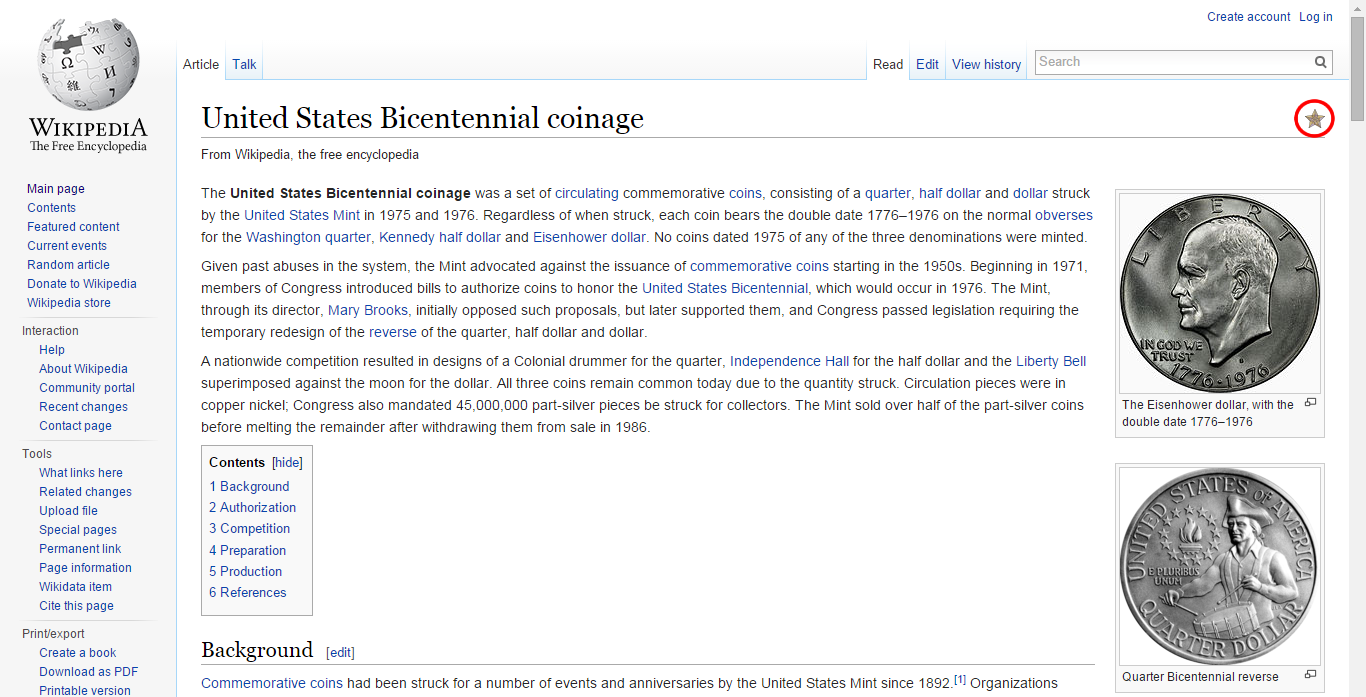
\includegraphics[width=1\textwidth]{imagenes/articulo_destacado1.png}
		\caption{Art\'iculo: United States Bicentennial Coinage (monedas del bicentenario de Estados Unidos). Extracto de un art\'iculo con la distinci\'on de art\'iculo destacado (se\~nalado con rojo). }
		\label{fig:usbicoinage}
	\end{center}
\end{figure}

Para clarificar lo nombrado en p\'arrafos anteriores acerca de art\'iculos destacados en otros idiomas, en la figura ~\ref{fig:estrellaamarilla}  podemos apreciar c\'omo un art\'iculo de la Wikipedia en Espa\~nol, nos indica a trav\'es de una estrella amarilla al lado de la palabra \emph{''English''}, que el mismo art\'iculo se encuentra en el idioma Ingl\'es y esa versi\'on corresponde a un art\'iculo destacado.

\begin{figure}[here]
	\begin{center}
		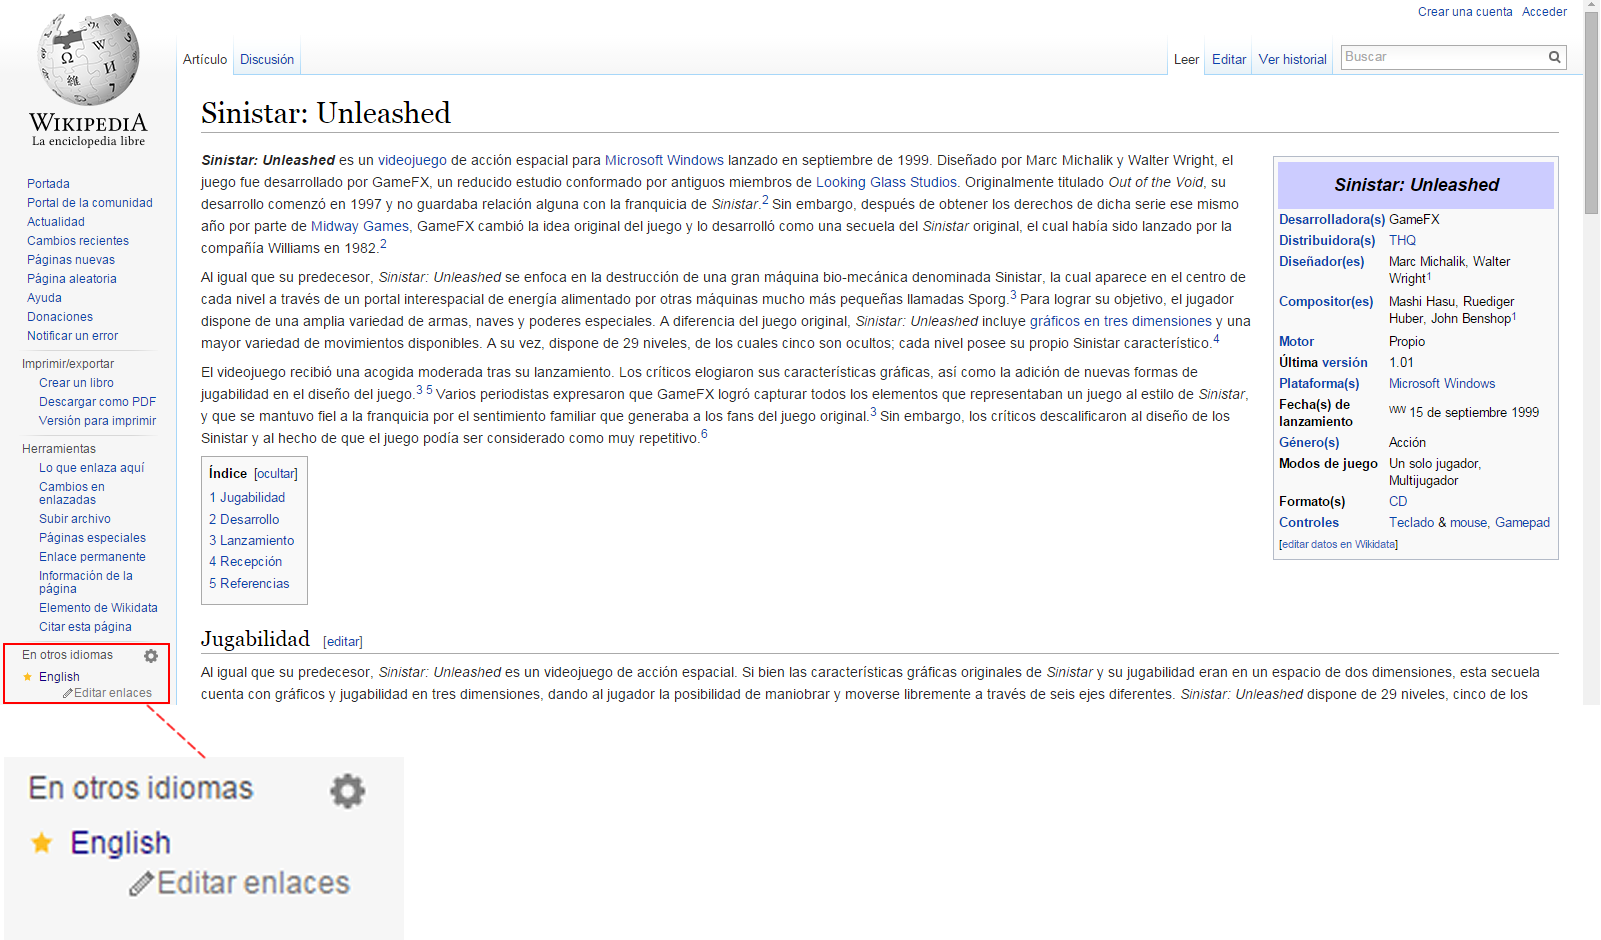
\includegraphics[width=1\textwidth]{imagenes/articulo_destacado3.png}
		\caption{Art\'iculo: Sinistar: Unleashed. Extracto de un art\'iculo con la distinci\'on de art\'iculo destacado (se\~nalado con rojo).}
		\label{fig:estrellaamarilla}
	\end{center}
\end{figure}

Actualmente, se cuenta con 4321 art\'iculos destacados en Ingl\'es de aproximadamente 3.454.284 . Esto indica que s\'olo el 0.1\% de los art\'iculos est\'a catalogado como FA.

Los criterios actuales que determinan un FA son: (1) completo; (2) preciso y verificable con fuentes; (3) estable; (4) bien escrito; (5) no controversial; (6) cumplir las normas de Wikipedia y gu\'ias de proyectos; (7) tener im\'agenes apropiadas; (8) tener longitud apropiada.

Profundicemos a continuaci\'on las caracter\'isticas nombradas aclaradas por Wikipedia\footnote{Criterios de Featured Articles. https://es.wikipedia.org/wiki/WP:QEUAD}.
\begin{itemize}
\item (1) Completo, implica que no omiten hechos, aspectos ni detalles importantes y que el art\'iculo tiene una extensi\'on adecuada sin perderse en detalles innecesarios, tratando con adecuada profundidad el tema.
\item (2) La informaci\'on debe ser precisa y verificable a trav\'es de referencias que muestre a quien se atribuye la sentencia. El art\'iculo debe estar basado en hechos y debe estar acompa\~nado de una lista de referencias que lo avalen.
\item (3) El art\'iculo no debe estar sometido a una guerra de ediciones constante ni modificar el contenido frecuentemente.
\item (4) El texto debe ser claro, conciso, convincente, sin faltas ortogr\'aficas, gramaticales o de estilo. El art\'iculo debe contener im\'agenes, tablas, gr\'aficos y otros elementos multimedia.
\item (5) El art\'iculo presentado, no debe contener citas que se contradigan o generen controversia. Los puntos de vista deben ser presentados sin sesgos y de manera justa.
\item (6) Debe cumplirse con el manual de estilo y seguir con la estructura formal de un art\'iculo, tales como un resumen conciso, tabla de contenidos, no contener v\'inculos a p\'aginas de desambiguaci\'on, etc.
\item (7) Las im\'agenes deben ser descriptivas y deben ser apropiadas,  intentando aclarar el contenido del art\'iculo.
\item (8) El art\'iculo no debe ser ni muy extenso ni muy corto, debe ser apropiado para expresar claramente la idea, con el nivel de detalle apropiado para el tema.
\end{itemize}

Un art\'iculo de Wikipedia debe someterse a un proceso para llegar a convertirse en FA. El mismo se convierte en destacado, luego de su nominaci\'on, revisi\'on y aprobaci\'on como art\'iculo candidato\footnote{Proceso de determinaci\'on de art\'iculos destacados \\ https://en.wikipedia.org/wiki/Wikipedia:Featured\_article\_candidates}. Los candidatos a art\'iculos destacados son revisados para determinar precisi\'on, neutralidad, integridad y estilo, de acuerdo a los criterios de los art\'iculos destacados nombrados anteriormente.

Aunque un art\'iculo destacado lleve tal distinci\'on, no significa que eventualmente pueda perderla. Esta situaci\'on puede darse por la introducci\'on de defectos debido a las diferentes ediciones que el art\'iculo sufra a lo largo del tiempo. Por este motivo, existe la Revalidaci\'on de Art\'iculos Destacados llamado RFA\footnote{Revalidaci\'on de Art\'iculos Destacados. \\ https://en.wikipedia.org/wiki/Wikipedia:Featured\_article\_review} (Review Featured Article), sistema por el cual permite acordar las correcciones que merece el art\'iculo.

Concentr\'emonos ahora en la tarea de diferenciar art\'iculos destacados de los que no lo son. La identificaci\'on de un art\'iculo destacado, es una tarea de clasificaci\'on binaria, que indica si el art\'iculo en cuesti\'on cumple o no las caracter\'isticas nombradas anteriormente. Definamos a continuaci\'on formalmente, en notaci\'on matem\'atica, a trav\'es de la siguiente funci\'on, la tarea de identificar art\'iculos destacados en Wikipedia.
\\

\textbf{Definici\'on 3: Identificaci\'on de un art\'iculo destacado.} Sea \emph{c} un clasificador, \emph{D} el conjunto de art\'iculos de Wikipedia, 0 y 1 valores enteros ($\mathbb{Z}$), la tarea de \emph{identificaci\'on de art\'iculos destacados}, es una funci\'on:

\begin{equation}
 \label{eq:ec1FFA}
\emph{c} :  \emph{D}  \rightarrow \emph{\{1,0\}}
\end{equation}

tal que \emph{c} es un clasificador que toma un art\'iculo de Wikipedia sobre el dominio \emph{D} y devuelve 1 en el caso de que el art\'iculo sea destacado o 0 en el caso que el art\'iculo no lo sea.

Luego de definir formalmente la tarea de identificaci\'on art\'iculos destacados y con el fin de seguir aclarando conceptos definidos en los p\'arrafos anteriores, veamos algunos ejemplos de este tipo de art\'iculos.

La figura ~\ref{fig:robinfriday} es un extracto de un art\'iculo destacado, acerca del futbolista profesional Ingl\'es Robin Friday nacido en el oeste de Londres, en el cual se muestra en el margen superior derecho, remarcado con un c\'irculo rojo, la estrella que indica que el mismo tiene el nivel de calidad m\'as alto en Wikipedia.

\begin{figure}[here]
	\begin{center}
		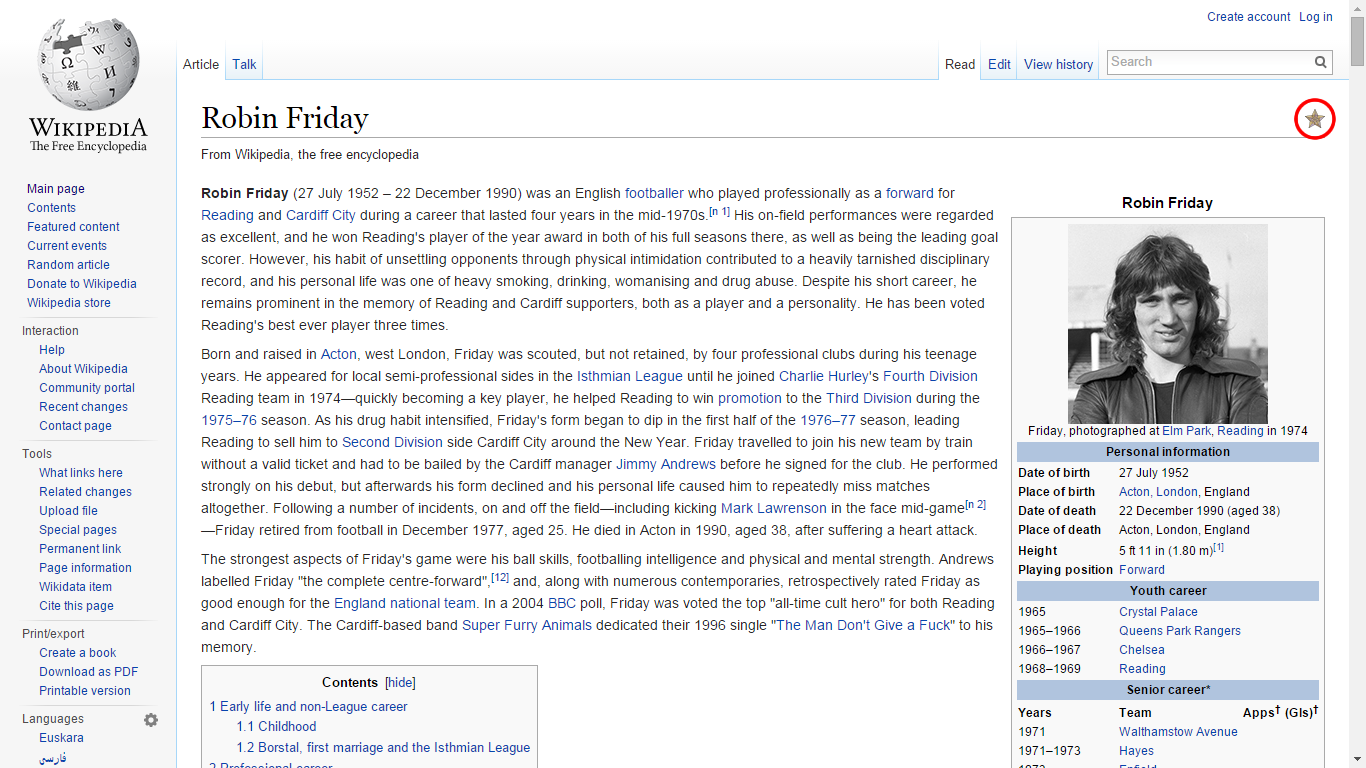
\includegraphics[width=1\textwidth]{imagenes/articulo_destacado.png}
		\caption{Art\'iculo: Robin Friday. Extracto de un art\'iculo con la distinci\'on de art\'iculo destacado (se\~nalado con rojo). }
		\label{fig:robinfriday}
	\end{center}
\end{figure}

Otro ejemplo de art\'iculo destacado, mostrado en la figura ~\ref{fig:sinistarunleashed}, podemos apreciarlo a trav\'es del art\'iculo \emph{Sinistar: unleashed}, correspondiente a un video juego de acci\'on de la empresa Microsoft presentado en el a\~no 1999. Tambi\'en, como se marc\'o en el ejemplo anterior, se indica con un c\'irculo rojo la estrella de bronce, categor\'ia de art\'iculo destacado para este art\'iculo de Wikipedia.

\begin{figure}[here]
	\begin{center}
		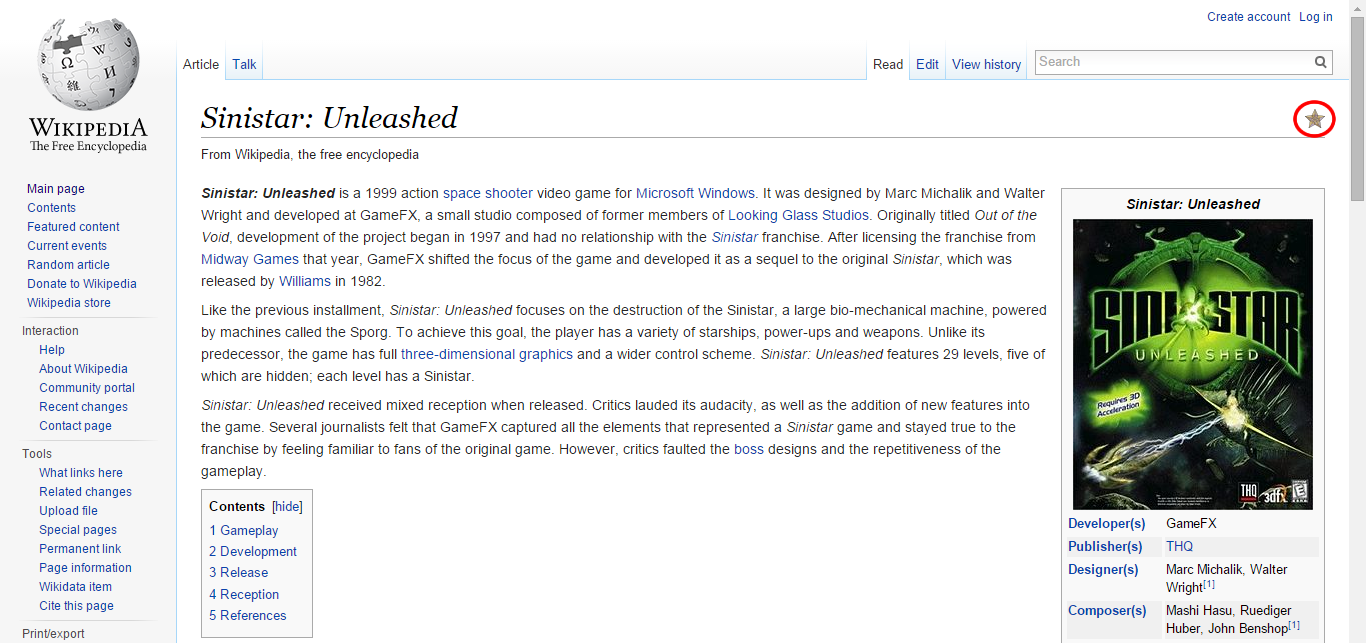
\includegraphics[width=1\textwidth]{imagenes/articulo_destacado2.png}
		\caption{Art\'iculo: Sinistar: Unleashed. Extracto de un art\'iculo con la distinci\'on de art\'iculo destacado (se\~nalado con rojo).}
		\label{fig:sinistarunleashed}
	\end{center}
\end{figure}

Wikipedia, afirma que provee una situaci\'on controlada respecto a la evaluaci\'on autom\'atica de la calidad de la informaci\'on, como fue se\~nalado en ~\cite{LiStei:10},  a trav\'es de la incorporaci\'on del concepto de art\'iculos destacados: “art\'iculos de alta calidad que son etiquetados de esa manera despu\'es de atravesar un extenso proceso de revisi\'on humana por pares” ~\cite{LiStei:10}. En pocas palabras, la comunidad de Wikipedia caracteriza como art\'iculos destacados aquellos que se distinguen por las normas profesionales de escritura, presentaci\'on, y el abastecimiento, los cuales se supone que poseen atributos espec\'ificos de calidad como bien escrito, amplio y bien investigado, neutral y estable como fue nombrado anteriormente.

En particular, la identificaci\'on autom\'atica de art\'iculos destacados (IFA) en Wikipedia es una tarea que ha ganado creciente inter\'es y ha sido abordada con diferentes enfoques. En el enfoque presentado por Blumenstock ~\cite{JoBl:08}, por ejemplo, sugiere utilizar simplemente el recuento de palabras como indicador de la calidad de los art\'iculos de Wikipedia. Sin embargo, en contraposici\'on, Lipka y Stein  ~\cite{LiStei:10} proponen otro m\'etodo sencillo y explotan la distribuci\'on de los trigramas de caracteres para identificar caracter\'isticas de alta calidad / buenos art\'iculos en Wikipedia.

Bas\'andonos en la interpretaci\'on de los metadatos, en el trabajo de ~\cite{WiHu:07} se presenta evidencia que los art\'iculos destacados pueden ser distinguidos de los no destacados a trav\'es del n\'umero de ediciones y editores, a mayor n\'umero de ediciones y editores,  mayor deber\'ia ser la calidad del art\'iculo.

Otra propuesta, que presenta una mirada desde un \'angulo similar, es el introducido por ~\cite{AnSmWi:09}, el cual no apunta a la medici\'on de los art\'iculos de Wikipedia, sin embargo, s\'i lo hace en la calidad de los contribuidores de Wikipedia. En este trabajo de investigaci\'on, detectaron que los usuarios registrados que hacen muchas contribuciones junto con contribuidores an\'onimos infrecuentes, generan contenido de alta calidad.

Como consecuencia del trabajo anterior, en ~\cite{LiRa:11}, se genera un aporte más importante, en el cual muestran c\'omo la calidad de Wikipedia no s\'olo depende de los diferentes tipos de contribuidores sino en c\'omo ellos colaboran entre s\'i.

Otros como ~\cite{WiHu:07} sostienen que la calidad de los art\'iculos est\'a estimada solamente con sus metadatos asociados sin requerir interpretaci\'on del contenido de los art\'iculos. Mientras que otros autores sostienen que cuando la identificaci\'on de art\'iculos destacados se realiza a trav\'es del an\'alisis del contenido, ~\cite{JoBl:08} es más apropiado realizar la medici\'on contando la cantidad de palabras en los art\'iculos.

Bas\'andose en el hecho de que los art\'iculos mas largos tienden a tener mas contenido factual, en un estudio propusieron la densidad factual ~\cite{LeVoErFeCaHoGrr:12}, con el fin de diferenciar art\'iculos destacados de art\'iculos que no lo son. Esta medida, relaciona la cantidad total de hechos del documento respecto a su longitud. Con este trabajo, se demostr\'o tambi\'en, que los art\'iculos destacados suelen ser m\'as informativos que los que no lo son, independientemente de su longitud ~\cite{PoFeErre:13}.

Por otro lado, otros trabajos presentaron enfoques diferentes y se basaron en simples estad\'isticas de los hechos obtenidos de los textos como la informaci\'on relacional contenida en los hechos y relaciones sem\'anticas como meronimia e hiperonimia entre otros ~\cite{LeVoErFeCaHoGrr:12}.

A pesar de la simplicidad (y eficacia) de los dos trabajos mencionados, en ~\cite{LeVoErFeCaHoGrr:12} se reconoce que para evaluar la precisi\'on factual del contenido de la Web, se requieren m\'as caracter\'isticas complejas sem\'anticas. Un enfoque com\'un es emplear extractores de informaci\'on abierta ~\cite{EtBaSoWe:12} o m\'etodos que utilizan conocimientos de fondo sobre relaciones sem\'anticas disponibles en recursos ontol\'ogicos como Wordnet ~\cite{Fel:98} y Yago ~\cite{StKaWe:07}. Estos enfoques extraen informaci\'on relacional acerca de las entidades nombradas en un texto particular (por ejemplo, hechos como f = (Mozart; naci\'o en; Salzburgo)). Adem\'as, se aprovechan las relaciones sem\'anticas definidas tales como meronimia e hiperonimia entre otras para inferir informaci\'on relacional entre entidades, que no se dan de forma expl\'icita en el texto.

A modo de aclaraci\'on y en contraposici\'on a los FA, el concepto de art\'iculo no destacado, desde ahora llamado NFA, representa un art\'iculo que no cumple con todas las caracter\'isticas de art\'iculo destacado (bien escrito, comprensivo, bien investigado, etc).

Vale destacar tambi\'en el concepto de un art\'iculo de Investigaci\'on Original (Original Research), desde ahora llamado OR, que surge de un documento que es una primera investigaci\'on, o est\'a escrito por los mismos investigadores que hicieron el estudio, con hip\'otesis o resultados reportados. Este conjunto de archivos corresponden a la colecci\'on de art\'iculos de investigaci\'on original del conjunto de entrenamiento suministrado en las competiciones PAN: Detecci\'on de Plagio, Autor Identificaci\'on, perfiles de autor\footnote{Competici\'on PAN. http://pan.webis.de/}. Esta colecci\'on cuenta con 506 archivos diferentes de Investigaci\'on Original y 939 de Art\'iculos no destacados.

\section{Detecci\'on de fallas en Wikipedia}

La detecci\'on de fallas de calidad en Wikipedia tiene como objetivo buscar imperfecciones de calidad espec\'ificas en los art\'iculos de la enciclopedia online. En otras palabras, las fallas, nos indican particularmente que una caracter\'istica del contenido debe ser modificada o agregada para mejorar su calidad y de esta manera no violar los est\'andares de calidad de Wikipedia.

\begin{table}
  \centering
   \begin{tabular}{ l l r }
	   \hline
	   & & \\
	   \textbf{Tipo de Falla} & \textbf{Descripci\'on de la Falla} & \textbf{Cantidad} \\ \\
	   \hline
     	   & & \\
	   Verificabilidad & Fuentes o referencias ausentes o & 98 \\
	   & inadecuadas  &  \\ \\
	   Estilo de escritura & No se ajusta al manual de estilo de & 74 \\
	   & Wikipedia  &  \\ \\
	   Miscel\'aneos & Fallas espec\'ificas, muy infrecuentes & 54 \\ \\
	   Temas espec\'ificos & Cuestiones que ocurren exclusivamente en & 44 \\
	   & ciertos temas &  \\ \\
	   Contenido no deseado & No se ajusta al criterio de inclusi\'on de & 42 \\
	   & Wikipedia &  \\ \\
	   Neutralidad & No escrito desde un punto de vista & 40 \\
	   & neutral &  \\ \\
	   Wiki tech & Cuestiones relacionadas a marcas, & 24 \\
	   & enlaces y categorizaci\'on &  \\ \\
	   Limpieza general & Problemas inespec\'ificos o generales & 17 \\ \\
	   Ampliar & Informaci\'on faltante o incompleta & 17 \\ \\
	   Estructura & Organizaci\'on inadecuada del contenido & 14 \\ \\
	   Sensibilidad al tiempo & Fuera de fecha o informaci\'on temporal no & 13 \\
	   & clara &  \\ \\
	   Unir & Contenido similar que debe ser combinado & 8 \\ \\
	  & & ---------- \\
 	  & & 445 \\
	\hline
 \end{tabular}
\caption {Los doce tipos de fallas generales con su respectiva descripci\'on y la cantidad de fallas de calidad que corresponden a ese tipo particular.}
\label{tablatfp1}
\end{table}

Para indicarles a los usuarios y editores de Wikipedia que un documento posee una falla de calidad en un art\'iculo o secci\'on, los usuarios de Wikipedia pueden optar por usar etiquetas de limpieza que se insertan dentro del documento llamadas \emph{cleanup tags}\footnote{Etiquetas de limpieza. https://en.wikipedia.org/wiki/Wikipedia:Cleanup}.

Las etiquetas pueden encontrarse en diferentes lugares del documento, ya que las fallas tienen como caracter\'istica que pueden tener diferentes alcances. Algunas fallas pueden referirse a todo el documento, por ejemplo indicando que \emph{faltan referencias} o simplemente a una secci\'on, indicando \emph{ampliar la secci\'on} o a\'un en otros casos, podemos encontrar reclamos particulares que indiquen, por ejemplo, que \emph{requiere una referencia} o que el \emph{v\'inculo se encuentra roto}. En el primero de los casos, encontramos la etiqueta al comienzo del documento de manera destacada, mientras que en el segundo se encuentra embebido en el texto.

Cabe destacar que en el snapshot correspondiente al 4 de enero de 2012 se identificaron 445 fallas de calidad en la Wikipedia en Ingl\'es  ~\cite{MaAn:13} y que las \emph{cleanup tags} son definidas por la comunidad de Wikipedia y pueden ser utilizadas por cualquier usuario.

La detecci\'on de dichas fallas de calidad, es usualmente considerada como un \emph{problema de clasificaci\'on de una clase}, donde para cada falla existente se construye un clasificador espec\'ifico para decidir si un art\'iculo de Wikipedia tiene dicha falla o no. A continuaci\'on definamos formalmente la falla de calidad en notaci\'on matem\'atica con el fin de clarificar los conceptos.\\

\textbf{Definici\'on 4: Detecci\'on de fallas de calidad.} Sea \emph{c} un clasificador, \emph{D} el conjunto de art\'iculos de Wikipedia, 0 y 1 valores enteros ($\mathbb{Z}$), la tarea de \emph{detecci\'on de fallas de calidad}, es una funci\'on:

\begin{equation}
 \label{eq:ec1FFC}
\emph{$c_{i}$} :  \emph{D}  \rightarrow \emph{\{1,0\}}
\end{equation}

tal que \emph{c} es un clasificador que toma un art\'iculo de Wikipedia sobre el dominio \emph{D} y devuelve 1 en el caso de que se identifique la falla \emph{i} en el art\'iculo o 0 en caso contrario.

Luego de definir formalmente la tarea de detecci\'on de fallas de calidad, a continuaci\'on veamos algunos ejemplos de fallas de calidad en Wikipedia que nos clarificar\'an los conceptos definidos anteriormente.

El art\'iculo de la Wikipedia en Ingl\'es que tiene como t\'itulo ``Murghazar''\footnote{Art\'iculo con fallas de calidad ``Murghazar''. https://en.wikipedia.org/wiki/Murghazar}, mostrado en la im\'agen ~\ref{fig:murghazar}, contiene diferentes fallas de calidad indicadas a trav\'es de etiquetas de limpieza. Al principio del documento, remarcado en rojo, encontramos una caja de etiquetas que nos indica que el documento tiene m\'ultiples cuestiones a corregir o mejorar. En primer lugar, el art\'iculo no cita fuentes o referencias. Adem\'as, el art\'iculo es hu\'erfano, lo que indica que no existen v\'inculos dentro de Wikipedia que lo enlacen. En \'ultimo lugar, se se\~nala que el art\'iculo esta escrito como si fuera publicidad. Tambi\'en, embebido en el texto, nos encontramos con etiquetas \emph{``[citation needed]''}, lo que nos indica que para esos fragmentos de texto, se necesitan citas que los avale.

\begin{figure}[here]
	\begin{center}
		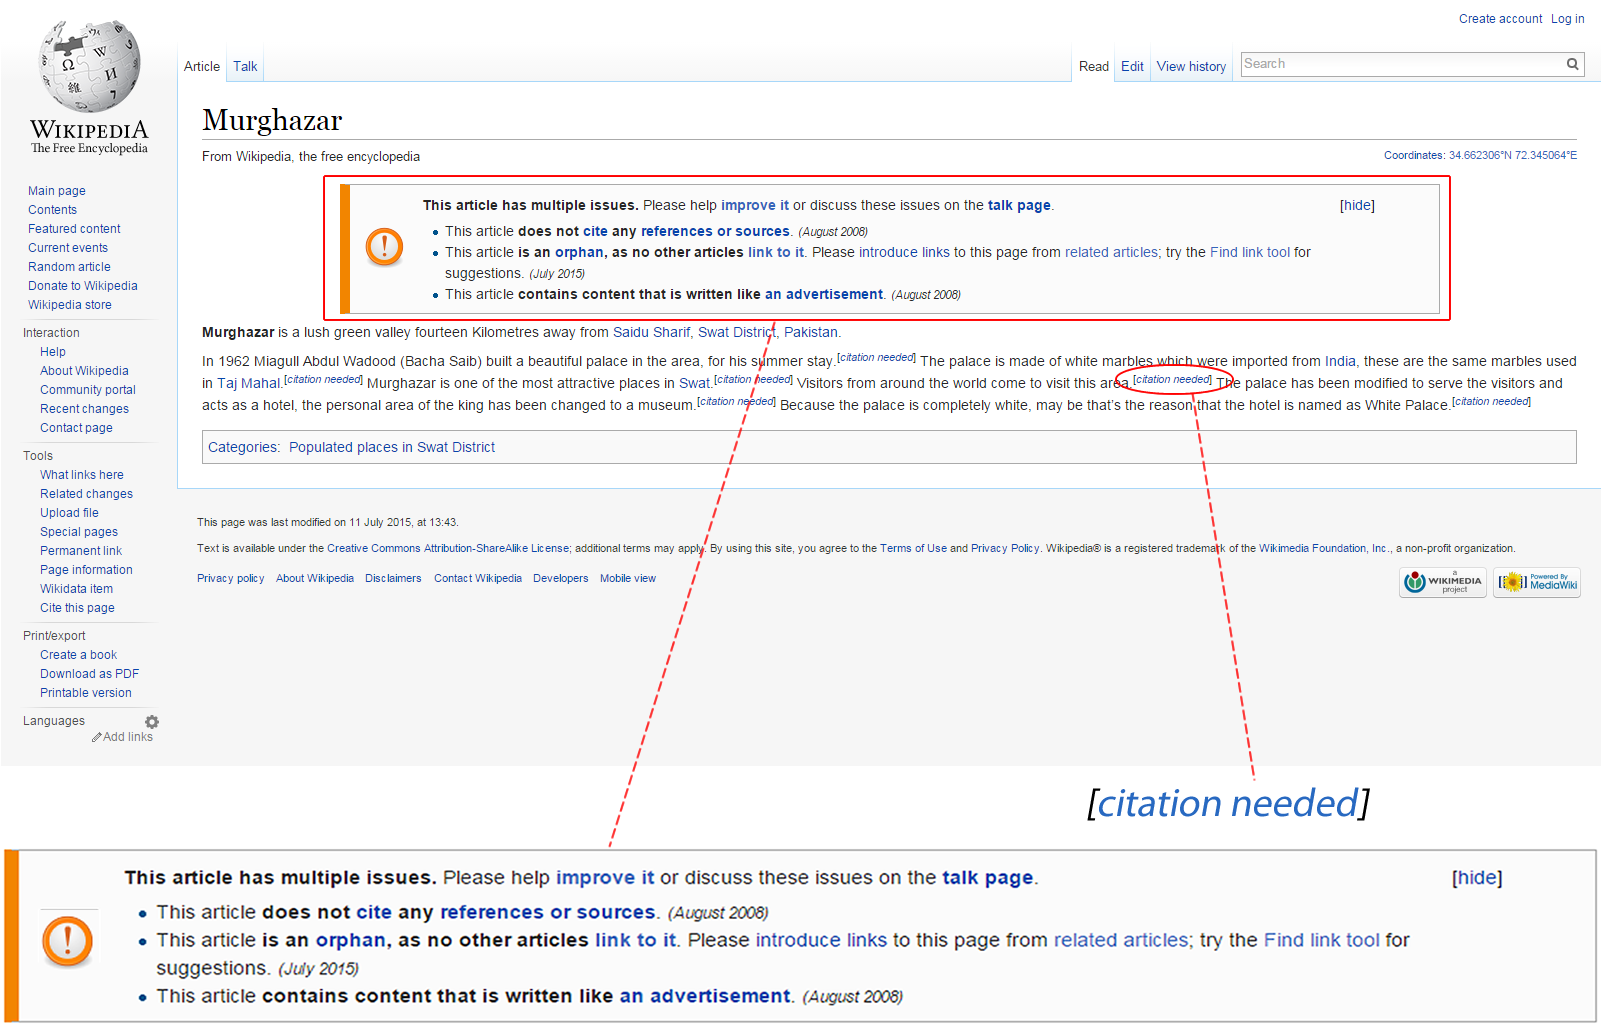
\includegraphics[width=1\textwidth]{imagenes/deteccion_falla.png}
		\caption{Art\'iculo de Wikipedia ''Murghazar'' con dos etiquetas de limpieza. La primera, ubicada al comienzo del art\'iculo indicando m\'ultiples cuestiones y la segunda, embebida en el texto indicando que faltan citas. }
		\label{fig:murghazar}
	\end{center}
\end{figure}

Otro ejemplo que muestra una falla diferente, podemos verlo en la figura ~\ref{fig:listgovernors}. Podemos apreciar el art\'iculo de la Wikipedia en Ingl\'es titulado ``List of Governors General of Canada''\footnote{Art\'iculo con fallas de calidad ``List of Governors General of Canada''. https://en.wikipedia.org/wiki/List\_of\_Governors\_General\_of\_Canada\#Governors\_ \\
General\_of\_the\_Province\_of\_Canada.2C\_1840.E2.80.931867} (lista de governadores generales de Canad\'a) en el cual se detectan falta de citas en ciertos fragmentos del texto indicandos\'e a trav\'es de la etiqueta \emph{``[citation needed]''}, y adem\'as, en el mismo art\'iculo, encontramos una caja de etiqueta en la secci\'on \emph{``Viceroys of Canada''} (\emph{``Virreyes de Canad\'a''}), que nos indica que esa secci\'on particular debe ser expandida o ampliada ya que se encuentra incompleta.

\begin{figure}[here]
	\begin{center}
		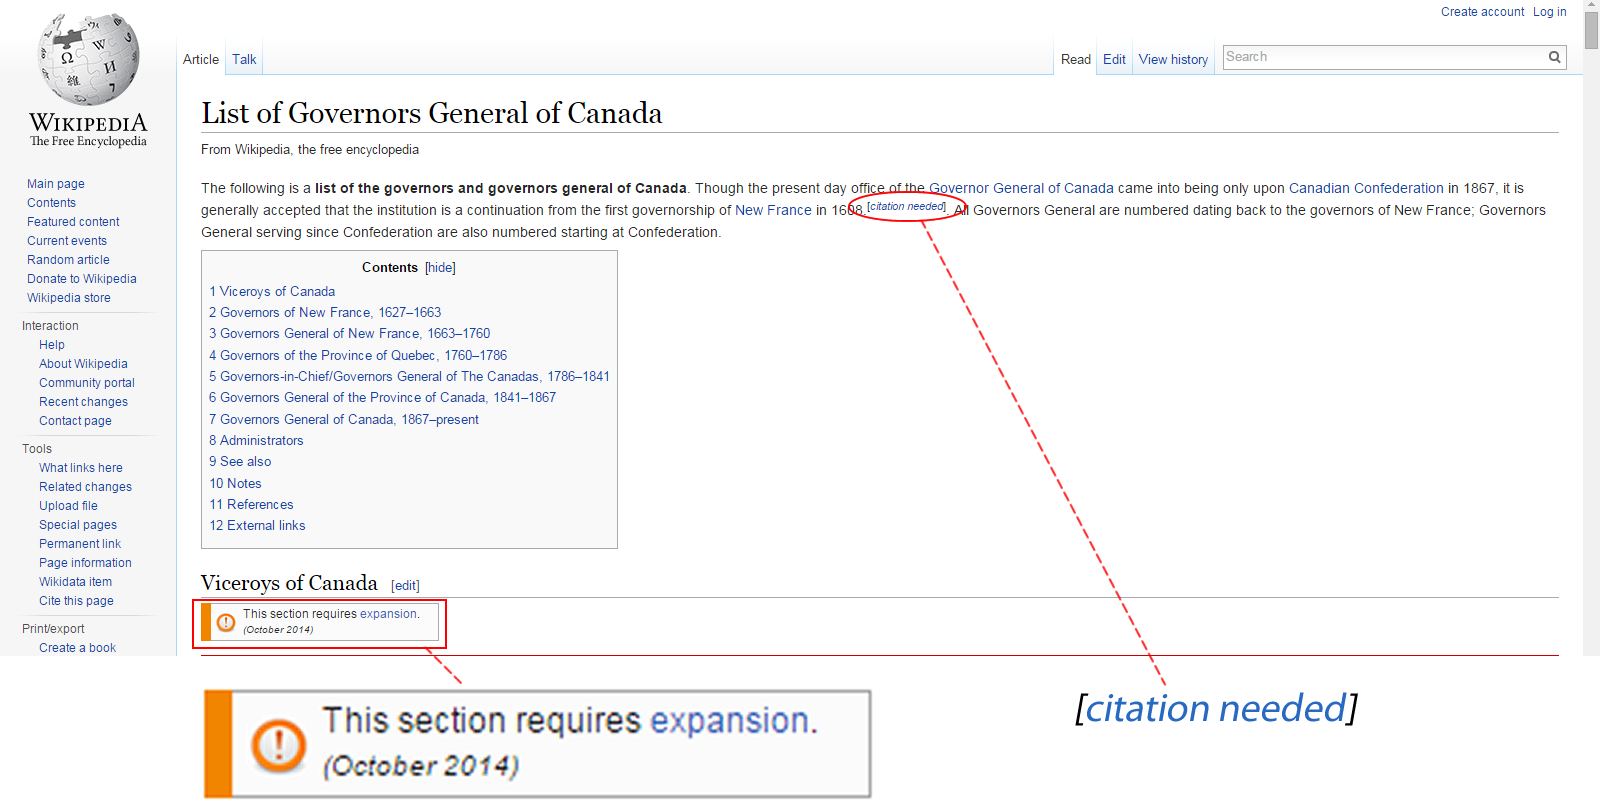
\includegraphics[width=1\textwidth]{imagenes/deteccion_falla2.png}
		\caption{Art\'iculo de Wikipedia ``List of Governors General of Canada'' con dos etiquetas de limpieza. Una indicando que una secci\'on debe ampliarse o mejorarse y otra embebida en el texto indicando que faltan citas. }
		\label{fig:listgovernors}
	\end{center}
\end{figure}

En la figura ~\ref{fig:hamptonwood}, como \'ultimo ejemplo, podemos apreciar el art\'iculo de la Wikipedia en Ingl\'es titulado ``Hampton Woods''\footnote{Art\'iculo con fallas de calidad ``Hampton Woods''.\\ https://en.wikipedia.org/wiki/Hampton\_Woods} en el cual al comienzo del art\'iculo se indica a trav\'es de una caja de etiquetas que posiblemente el art\'iculo contiene investigaci\'on original, ya que no existen fuentes que avalen la informaci\'on. Tambi\'en, inmediatamente debajo, se indica que no se citan referencias o fuentes.

\begin{figure}[here]
	\begin{center}
		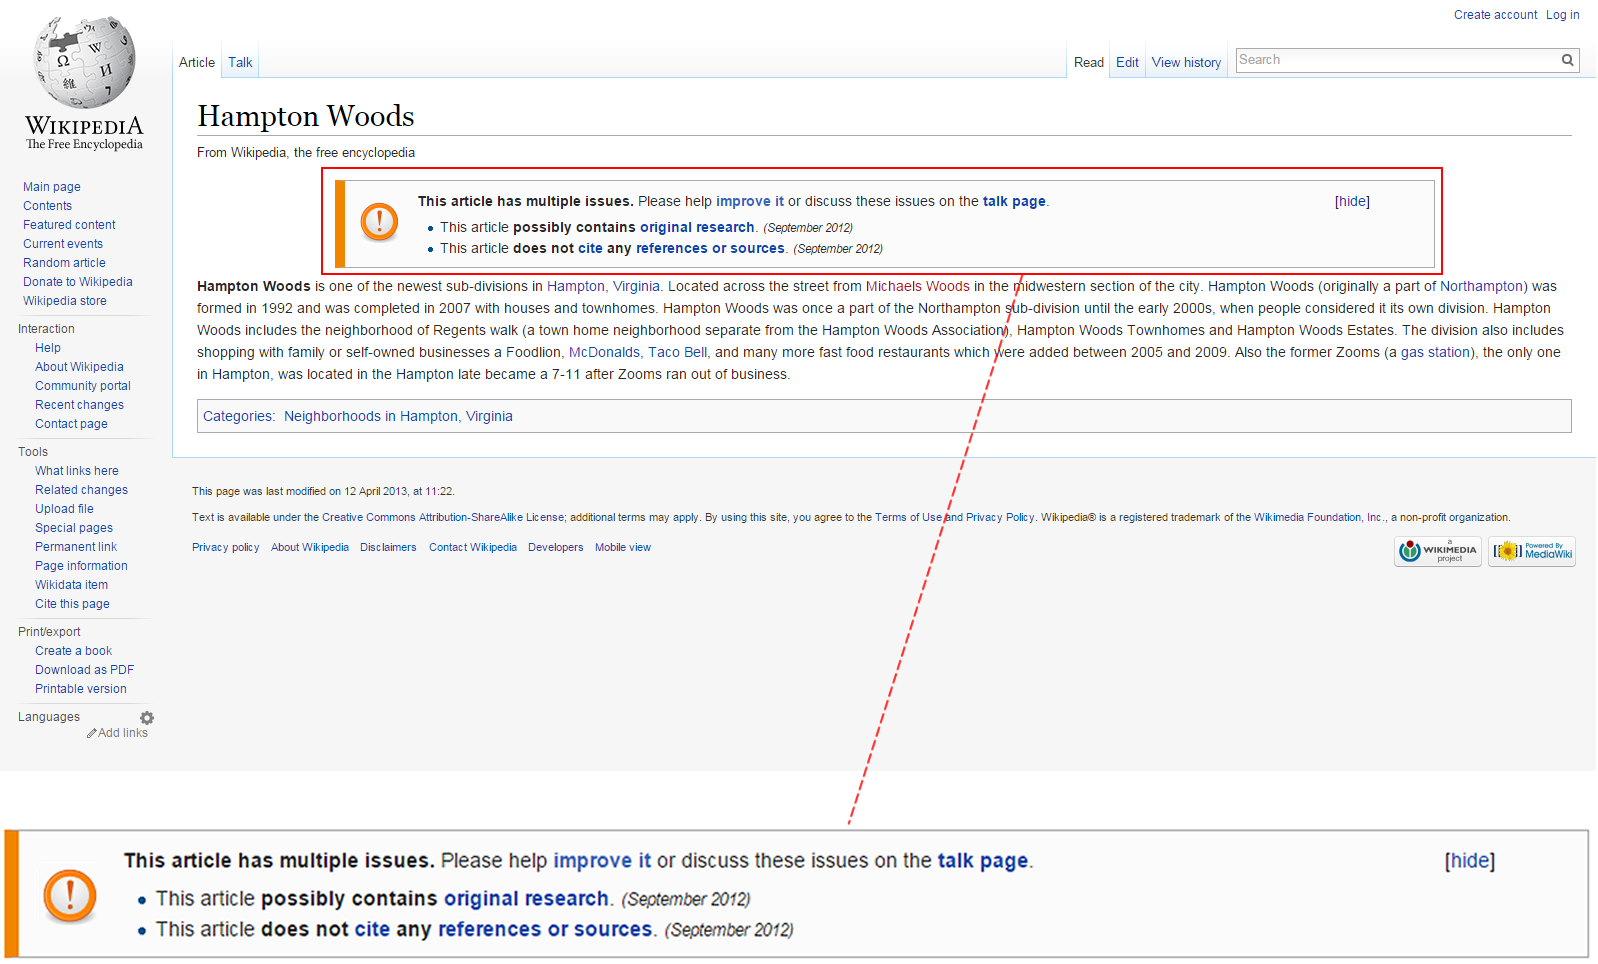
\includegraphics[width=1\textwidth]{imagenes/deteccion_falla3.png}
		\caption{Art\'iculo de Wikipedia ``Hampton Woods'' con la etiqueta \emph{investigaci\'on original} y \emph{falta de fuentes} }
		\label{fig:hamptonwood}
	\end{center}
\end{figure}

Si bien existen investigaciones que consideraron peque\~nas muestras de art\'iculos ~\cite{StTwSmGa:08} o analizaron un conjunto restringido de fallas de calidad ~\cite{AndSteLip:11, GaBeRoDa:09}, los pioneros en realizar un an\'alisis detallado fueron investigadores de la Universidad de Weimar, encabezado por Mike Anderka ~\cite{AndSte:10, AndSteBu:12, AndSteLip:12}. Este estudio revel\'o que un 27.52 \% de los art\'iculos de Wikipedia en Ingl\'es contiene al menos una falla de calidad y que un 70 \% corresponde a deficiencias de verificabilidad. Como se basaron en art\'iculos etiquetados manualmente, el porcentaje real, tiende a ser m\'as alto que el nombrado, por lo que existe la posibilidad de que muchos art\'iculos con deficiencias no hayan sido identificados todav\'ia ~\cite{PoFeErre:13}.

En el trabajo llevado a cabo por ~\cite{MaAn:13} se agrupan las 445 fallas nombradas anteriormente en 12 categor\'ias ya que varias fallas se relacionan al mismo tipo, por ejemplo, \emph{no referenciada} y \emph{necesita citas}, ambas se refieren a verificabilidad, una categor\'ia que hace alusi\'on a un documento que no presenta referencias. Como aporte principal de este trabajo, se propone una miner\'ia autom\'atica para extraer las etiquetas de limpieza de Wikipedia, las cuales nos dan el conjunto completo de las fallas de calidad identificadas por los usuarios de Wikipedia.  Esta organizaci\'on revela la estructura de las fallas de calidad de Wikipedia as\'i como tambi\'en indica la importancia de la misma.

En el cuadro ~\ref{tablatfp1} se muestra el agrupamiento de fallas determinado en dicha investigaci\'on,  su descripci\'on y cantidad de fallas de calidad relacionadas. A continuaci\'on se explican los 12 agrupamientos.

El primero, \emph{verificabilidad}, es uno de los principios m\'as importantes de una enciclopedia, y hace referencia a art\'iculos que no tienen referencias (\emph{sin referencias}, \emph{sin notas al pie de p\'agina}), son inadecuadas o inv\'alidas (\emph{fuentes primarias}, \emph{v\'inculo roto}) o simplemente que tienen declaraciones sin fuentes (\emph{necesita citas}, \emph{qui\'en} y \emph{por qui\'en}).

La falla \emph{estilo de escritura}, se refiere a caracter\'isticas estil\'isticas como gram\'atica, estilo, cohesi\'on, tono, etc, la mayor\'ia detallados en el manual de estilos de Wikipedia\footnote{Manual de estilos de Wikipedia. http://en.wikipedia.org/wiki/Wikipedia:Manual\_of\_Style.}.

El agrupamiento bajo el nombre \emph{miscel\'aneos}, comprende fallas que son muy espec\'ificas y que ocurren infrecuentemente.

Las fallas que surgen en un tema particular, se organizan bajo el tipo \emph{tema espec\'ifico}. Por ejemplo, la falla \emph{plot}, argumento, indica que el argumento de resumen podr\'ia ser muy extenso o excesivamente detallado, que s\'olo aplica a pel\'iculas o novelas.

La falla \emph{contenido no deseado} se refiere al contenido que no es apropiado por una enciclopedia (\emph{notabilidad}, \emph{publicidad}, \emph{investigaci\'on original}).

La falla \emph{neutralidad}, hace referencia a que el contenido es imparcial y sin opiniones, un elemento muy importante para una enciclopedia.

\emph{Wiki tech}, otro de los agrupamientos, hace alusi\'on a aspectos t\'ecnicos del art\'iculo, por ejemplo, que sea hu\'erfano, es decir, que no haya referencias a \'el o que no est\'e categorizado.

La falla \emph{limpieza general} agrupa las etiquetas de limpieza que listan varias fallas en una sola etiqueta (\emph{m\'ultiples cuestiones}) o simplemente requieren de una limpieza sin proveer mayor informaci\'on.

La falla \emph{ampliar}, indica que deben mejorarse ciertas secciones completando con mayor detalle o que cierta informaci\'on falta.

La falla \emph{estructura} nos determina que los art\'iculos deben estar organizados en secciones y con ciertas longitudes, etc.

Aquellos art\'iculos que est\'en determinados por el tiempo de vida o la actualidad deben estar organizados bajo la falla \emph{sensibilidad al tiempo}. Por \'ultimo, los art\'iculos que manejen temas similares deben ser combinados bajo la falla \emph{unir}.

De las 445 fallas de calidad, el trabajo nombrado se enfoca en las 10 fallas principales de la Wikipedia en Ingl\'es:
\begin{itemize}
\item 	No Referenciado: el art\'iculo no cita referencia o fuentes.
\item 	Hu\'erfano: se tiene menos de 3 enlaces entrantes en el art\'iculo.
\item 	Mejora de referencias: el art\'iculo necesita referencias adicionales para su verificaci\'on.
\item 	Secci\'on vac\'ia: el art\'iculo al menos tiene una secci\'on vac\'ia.
\item 	Notabilidad: el art\'iculo no cumple con la directriz general de notabilidad.
\item 	Sin nota de pie: no posee notas al pie de p\'agina.
\item 	Fuentes primarias: el art\'iculo se basa en referencias a las fuentes primarias.
\item 	Wikifi: el art\'iculo necesita ser wikificado (enlaces internos y  el dise\~no).
\item 	Anuncio: el art\'iculo est\'a escrito como un anuncio.
\item 	Investigaci\'on original: el art\'iculo contiene una investigaci\'on original.
\end{itemize}

En el estudio nombrado, se intent\'o determinar si un art\'iculo contiene o no una falla de calidad, dada una muestra de art\'iculos que contienen dicha falla. Se trat\'o el problema como uno de clase \'unica con el m\'etodo PU Learning (aprendizaje de ejemplos positivos y no etiquetados). Dicho m\'etodo utiliza un peque\~no conjunto de clases etiquetadas positivas, ninguna negativa (siendo \'este el mayor desaf\'io planteado) y un gran conjunto no etiquetado para ayudar a un modelo que se utiliza para predecir la presencia o no de la falla.

A modo de conclusi\'on, en los trabajos encabezados por Mike Anderka, se aborda la idea de fallas de calidad desde una perspectiva diferente a trav\'es del uso de etiquetas de limpieza, los cuales son indicadores de calidad de los art\'iculos, como se detall\'o en p\'arrafos anteriores. En una primera investigaci\'on ~\cite{AndSte:10} provee un desglose de las fallas de calidad de la Wikipedia en Ingl\'es, mientras que eval\'uan su eficacia para garantizar la calidad en ~\cite{AndSteBu:12} mediante el an\'alisis de la evoluci\'on de marcadores de fallas de calidad en el tiempo. Por \'ultimo, en ~\cite{AndSteLip:12}, los autores logran detectar autom\'aticamente fallas de calidad a trav\'es de la predicci\'on de etiquetas de limpieza en art\'iculos no vistos, lo cual coincide con la tarea planteada como objetivo en el desaf\'io PAN.

En la investigaci\'on ~\cite{OfIgMr:12} se propone un m\'etodo diferente, en \'el construyen un sistema llamado \emph{FlawFinder}, un sistema modular y flexible para predecir autom\'aticamente fallas de calidad en art\'iculos de Wikipedia a trav\'es de cinco componentes los cuales podr\'ian trabajar de manera independiente tambi\'en; un lector de corpus, un preprocesador, una unidad de extracci\'on de caracter\'isticas, un m\'odulo para entrenamiento y un escritor de reportes.

Como caracter\'istica destacable de este trabajo de investigaci\'on, \'este sistema, en vez de leer los datos de entrenamiento proporcionados por la competencia PAN, en la cual obtuvo la mejor precisi\'on de todos los sistemas expuestos y el segundo puesto en cuanto a recall y F1, directamente el lector de corpus accede a los art\'iculos desde a la base de Wikipedia creada por ellos mismos, la cual posee un amplio rango de meta datos tales como estructura de v\'inculos e informaci\'on acerca del historial de revisi\'on de los art\'iculos ~\cite{OfIgMr:12}.

\section{Visualizaci\'on} 